
% !TEX program = xelatex
\documentclass[12pt, a4paper]{report}


\usepackage{pifont}
% Suport pentru diacritice și alte simboluri
\usepackage{fontspec}

% Font Times New Roman
\usepackage{newtxtext} 

% Suport pentru mai multe limbi
\usepackage{polyglossia}

% Setează limba textului la română
\setdefaultlanguage{romanian}
% Am nevoie de engleză pentru rezumat
\setotherlanguages{english}

% Indentează și primul paragraf al fiecărei noi secțiuni
\SetLanguageKeys{romanian}{indentfirst=true}

% Suport pentru diferite stiluri de ghilimele
\usepackage{csquotes}

\DeclareQuoteStyle{romanian}
  {\quotedblbase}
  {\textquotedblright}
  {\guillemotleft}
  {\guillemotright}

% Utilizează biblatex pentru referințe bibliografice
\usepackage[
    maxbibnames=50,
    sorting=nty
]{biblatex}

\addbibresource{bibliography.bib}

% Setează spațiere inter-linie (doublespacing din LaTeX este echivalentul setarii 1.5 in Microsoft Word)
\usepackage{setspace}
\doublespacing
\usepackage{tgtermes}
% Modificarea geometriei paginii (cu margini de 2,5 cm) 
\usepackage[margin=2.5cm]{geometry}

% Include funcțiile de grafică
\usepackage{graphicx}
\usepackage{wrapfig}
% Încarcă imaginile din directorul `images`
\graphicspath{{./images/}}

% Listări de cod
\usepackage{listings}

% Linkuri interactive în PDF
\usepackage[
    colorlinks=true,
    linkcolor={black},
    menucolor={black},
    citecolor={black},
    urlcolor={black}      % black globally
]{hyperref}

\usepackage{biblatex}

% Switch URL color to blue only inside the bibliography
\AtBeginBibliography{\hypersetup{urlcolor=blue}}

% Simboluri matematice codificate Unicode
\usepackage[warnings-off={mathtools-colon,mathtools-overbracket}]{unicode-math}

% Comenzi matematice
\usepackage{amsmath}
\usepackage{mathtools}

% Formule matematice
\newcommand{\bigO}[1]{\symcal{O}\left(#1\right)}
\DeclarePairedDelimiter\abs{\lvert}{\rvert}

% Suport pentru rezumat în două limbi
% Bazat pe https://tex.stackexchange.com/a/70818
\newenvironment{abstractpage}
  {\cleardoublepage\vspace*{\fill}\thispagestyle{empty}}
  {\vfill\cleardoublepage}
\renewenvironment{abstract}[1]
  {\bigskip\selectlanguage{#1}%
   \begin{center}\bfseries\abstractname\end{center}}
  {\par\bigskip}

% Suport pentru anexe
\usepackage{appendix}

% Stiluri diferite de headere și footere
\usepackage{fancyhdr}

% Metadate
\title{Titlul lucrării de licență}
\author{Numele studentului}

% Generează variabilele cu @
\makeatletter

% Pachet pentru formatarea titlurilor de capitole și secțiuni
\usepackage{titlesec}

% Redefinirea formatului pentru \chapter pe un singur rând
\titleformat{\chapter}[block]
  {\normalfont\huge\bfseries}{\chaptername~\thechapter.}{15pt}{\Huge}

% Opțional: Ajustarea spațiului de deasupra și dedesubtul titlului
\titlespacing*{\chapter}{0pt}{-20pt}{40pt}

\begin{document}

% Front matter
\cleardoublepage
\let\ps@plain

% Pagina de titlu
\include{0-title}
\restoregeometry
\newgeometry{
    margin=2.5cm
}

\fancypagestyle{main}{
  \fancyhf{}
  \renewcommand\headrulewidth{0pt}
  \fancyhead[C]{}
  \fancyfoot[C]{\thepage}
}

\addtocounter{page}{1}

% Rezumatul
\begin{abstractpage}

\begin{abstract}{romanian}
Lucrarea de licență prezintă proiectarea și implementarea unei aplicații web pentru planificarea itinerariilor turistice, realizată cu ASP.NET Core MVC și Entity Framework Core. Sistemul permite utilizatorilor autentificați să creeze călătorii, să adauge locații și rezervări, să gestioneze tipuri de obiective prin etichete și să genereze automat planuri zilnice de vizitare.

Generatorul de itinerariu construiește agenda fiecărei zile pe baza datei de început și de sfârșit, orei de explorare, rezervărilor existente și duratei medii de vizitare pentru fiecare locație. Algoritmul prioritizează întâi evenimentele programate, apoi adaugă obiective disponibile din listă în ordinea proximității și a compatibilității cu intervalele orare. Lucrarea detaliază construcția modelelor de date relaționale, configurarea entităților many-to-many, validarea datelor și optimizarea fluxului de creare a itinerariului.

Rezultatul este o aplicație care sprijină utilizatorii în organizarea eficientă a traseelor turistice, sinteza rezervărilor și planificarea responsabilă a zilelor de vizitare, oferind o experiență coerentă pe tot parcursul procesului.
\end{abstract}

% \begin{abstract}{english}
% This bachelor's thesis presents the design and implementation of a web application for travel itinerary planning, built with ASP.NET Core MVC and Entity Framework Core. The system enables authenticated users to create trips, add locations and reservations, manage categories of attractions through tags, and automatically generate daily visit plans.

% The itinerary generator builds each day's schedule based on trip dates, exploration hours, existing reservations, and the average visit duration for each location. The algorithm prioritizes scheduled events first, then adds available attractions by proximity and time window compatibility. The thesis details the construction of relational data models, many-to-many entity configuration, input validation, and itinerary generation flow optimization.

% The result is an application that supports users in organizing travel routes efficiently, combining bookings and daily planning into a cohesive experience throughout the trip preparation process.
% \end{abstract}

\end{abstractpage}

\tableofcontents

% Main matter
\cleardoublepage
\pagestyle{main}
\let\ps@plain\ps@main

\chapter{Introducere}

\section{Motivație}
Mereu am fost pasionată de călătorii și de organizarea acestora. În era digitală actuală, am observat că există o multitudine de aplicații care oferă informații turistice, care își oferă posibilitatea de a face liste cu destinații sau care marchează destinațiile pe hartă. Insă puține dintre ele se concentrează pe planificarea detaliată a itinerariilor. 

Mi-am dorit să creez o soluție care să ajute utilizatorii să-și organizeze eficient traseele turistice, să aibă posibilitatea de a adăuga rezervări și să ofere un plan zilnic coerent pentru a maximiza experiența de călătorie.

Motivația mea este de a inspira cât mai mulți oameni să descopere diversitatea lumii, sa viziteze cât mai mult fără stresul organizării.

\section{Nevoi pe care aplicația le satisface}
Scopul principal al aplicatiei este de a veni in sprijinul pasionaților de calatorii care nu au timpul necesar sau cărora, pur si simplu, nu le face plăcere procesul de organizare. Aplicația elimină complet efortul de a căuta informații pe site-uri reducând oboseala planificării. Prin preluarea acestei etape utilizatorul se poate axa explusiv pe relaxare si vizitarea țării respective.

Pentru o eficientizare maximă, platforma este concepută să se adapteze stilului fiecărui utilizator. Acesta poate adăuga manual destinații si rezervări pe care le-a făcut deja, sau poate lăsa aplicația să genereze partial sau total itinerariul. Pentru a crea un plan automatizat si personalizat, preferintele sunt colectate într-un mod practic si interactiv: utilizatorul sortează o lista de categorii si le sortează pe trei nivele de prioritate. Astfel traseul generat se va mula pe interesele utilizatorului. 

Nu în ultimul rând, aplicația rezolvă problema centralizării informațiilor. Prin crearea unui cont personalizat utilizatorii scapa de grija rezervărilor, adreselor si notitelor. Totul este adunat intr-un spatiu clar. Din secțiunea principală acesta poate vizualiza si gestiona rapid călătoriile curente sau viitoare (cat si cele trecute). În plus, pentru un ton mai interactiv interfața integrează un calendar în care perioadele de vacanță sunt evidențiate alaturi de o hartă interactiva în care sunt evidențiate țarile explorate.

\section{Aplicații similare}
\ding{117} Google Maps

„Google Maps” este o aplicație destinată căutării de locații și calculării direcțiilor între diferite puncte de interes. Funcționarea acesteia se bazează pe utilizarea unui cont Google asociat, oferind utilizatorului posibilitatea de a căuta destinații atât după denumire și coordonate, cât și prin selectarea dintr-o anumită categorie de interes (restaurante, atracții etc.).

O funcționalitate importantă este posibilitatea de a salva locațiile preferate în liste individuale, facilitând organizarea personalizată. De asemenea, aplicația permite calcularea rutelor între mai multe puncte de oprire. Totuși, un dezavantaj în planificarea itinerariilor complexe este faptul că ordinea locațiilor nu este optimizată automat, aceasta trebuind să fie stabilită manual, uneori în mod aleatoriu, de către utilizator.

\ding{117} Wanderlog

„Wanderlog” este o aplicație de planificare a călătoriilor ce permite utilizatorilor adăugarea de destinații, unități de cazare și atracții turistice, pe care le integrează și le plasează pe o hartă interactivă. Pentru a eficientiza organizarea traseului, aplicația calculează în mod automat distanțele și timpul de deplasare necesar între obiectivele selectate.

Deși oferă funcționalități utile organizării, experiența utilizatorului poate fi afectată de prezența diverselor sfaturi afișate constant sub formă de ferestre de tip pop-up, care pot deveni deranjante pe parcursul utilizării. De asemenea, un aspect limitativ este faptul că aplicația condiționează accesul la foarte multe acțiuni și funcții avansate de achiziționarea unei subscripții plătite.

\ding{117} Roamy

„Roamy” este o aplicație dedicată creării de itinerarii, disponibilă în prezent exclusiv în magazinul de aplicații Apple Store. La inițierea unei noi planificări, utilizatorul trebuie să introducă destinația dorită și numărul de zile alocate călătoriei. Ulterior, traseul poate fi construit fie prin adăugarea manuală a locațiilor, fie generat automat cu ajutorul funcțiilor bazate pe inteligență artificială.

Similar altor aplicații din această categorie, versiunea gratuită prezintă anumite restricții. Pentru a debloca toate funcționalitățile oferite de platformă și pentru a beneficia de o experiență de utilizare continuă, fără întreruperi cauzate de afișarea reclamelor, este necesară plata unui abonament lunar sau anual.


\section{Ce aduce nou}

În ceea ce privește noutățile și avantajele aduse față de alte soluții existente pe piață, aplicația se distinge în primul rând printr-un algoritm de recomandare personalizat. Spre deosebire de alte platforme care se limitează la a sugera cele mai vizitate atracții dintr-un oraș, acest algoritm utilizează un sistem avansat de selecție bazat pe preferințele reale ale utilizatorului. Aceste date sunt colectate într-un mod practic și interactiv: utilizatorul ordonează o listă de categorii de interes, încadrându-le în trei niveluri distincte de prioritate. Mai mult, algoritmul oferă flexibilitatea de a genera itinerariul fie integral, fie parțial, completând inteligent lista de locații deja adăugate manual de către utilizator, în cazul în care acestea nu sunt suficiente pentru a acoperi programul unei zile întregi.

Un alt avantaj major în organizarea logistică este serviciul de adăugare a unității de cazare ca punct oficial de pornire. Această funcționalitate contribuie la o calculare mult mai precisă a traseului zilnic, luând în considerare distanța și timpul exact de deplasare de la cazare până la prima destinație. În completarea acestei funcții, aplicația oferă posibilitatea de a integra rezervări prestabilite direct în itinerariu. Aceste evenimente primesc automat cel mai înalt grad de importanță, iar pentru a asigura respectarea programului, sistemul calculează și adaugă o marjă de eroare temporală - ascunsă în interfața utilizatorului - garantând astfel sosirea la timp la rezervările efectuate.

Pe parcursul desfășurării călătoriei, aplicația permite un management dinamic al traseului prin actualizări în timp real. Utilizatorul are posibilitatea de a bifa locațiile vizitate, iar în cazul în care anumite obiective din program nu au putut fi atinse în zilele anterioare, sistemul oferă opțiunea de a regenera itinerariul, reprogramând inteligent locațiile rămase. 

Nu în ultimul rând, având ca scop principal facilitarea planificării și transformarea călătoriei într-o experiență memorabilă, aplicația integrează elemente specifice de gamificare. Printre acestea se numără teste cu întrebări de cultură generală despre destinații, o hartă interactivă pe care țările vizitate sunt evidențiate cromatic, precum și un calendar vizual unde utilizatorii își pot urmări cu ușurință istoricul călătoriilor.

\section{Structura lucrării}

Această lucrare este structurată în patru capitole, fiecare servind un rol specific în prezentarea temei abordate:

\begin{itemize}
    \item Introducere: Oferă o privire de ansamblu asupra subiectului, motivația mea, nevoi pe care aplicația le satisface, o privire de ansamblu a aplicațiilor similare adăugând ce îmbunătățiri am adus eu
    \item Tehnologii și framework-ul utilizat: este structurat pe subcapitole dedicat fiecărei tehnologii utilizate
    \item Prezentarea aplicației: prezintă întreaga funcționalitate a aplicației, din perspectiva unui utlizator obișnuit. Fiecarui subcapitol îi este asociat o pagina cu feature-urile asociate
    \item Concluzia: sunt reunite concluziile și perspectivele de dezvoltare ale aplicației.
\end{itemize} 
\chapter{Tehnologii și Framework-uri utilizate}

\section{Framework Backend: .NET and ASP.NET Core}

\subsection{Ecosistemul C\# si .NET 8}
Alegerea folosirii limbajului C\# și a platformei .NET 8 a fost motivată de necesitatea unui ecosistem robust, capabil să susțină o logică de business complexă pentru aplicații de tip întreprindere.Aplicația impune implementarea unor algoritmi avansați pentru orchestrarea datelor, după cum urmează:

\begin{itemize}
    \item  \textbf{Optimizarea algoritmică a itinerariului:} implică rezolvarea unor variații ale problemei comis-voiajorului și aplicarea unor euristici de rutare. Sistemul calculează traiectoriile optime între locații (noduri) multiple, respectând riguros constrângerile multidimensionale de distanță fizică și ferestrele de timp.
    \item  \textbf{Mecanisme de potrivire:} presupun filtrarea avansată și ierarhizarea ponderată a punctelor de interes. Algoritmul procesează preferințele utilizatorului pe trei nivele de prioritate, realizând o mapare semantică între locații și vectorul de preferințe.
    \item  \textbf{Programarea temporală:} soluționarea unor probleme de satisfacere a constrângerilor pentru alocarea și gestionarea intervalelor zilnice, asigurând crearea unor planificări fără suprapuneri, cu timpi de tranzit calculați și cu o marjă de siguranță pentru rezervări, acestea având cea mai mare prioritate.

\end{itemize}

C\# oferă avantajul verificării statice a tipurilor la compilare (static type checking) și al un sistem de tipuri puternice (strong type). Aceste caracteristici scad semnificativ riscul excepțiilor la execuție (runtime exceptions) și garantează integritatea memoriei, un atribut critic pentru consistența funcțională a aplicației.

În plus, trecerea la .NET 8 introduce optimizări la nivel de execuție, îmbunătățiri ale compilatorului JIT (Just-in-Time) și opțiuni de compilare AOT (Ahead of Time)\href{https://medium.com/@Mr.Jafri_01/just-in-time-jit-vs-ahead-of-time-aot-compilation-in-net-core-c7650f1a366a}{}\cite{jitAOT_ref}. Acestea se traduc printr-un timp de inițializare extrem de redus și o amprentă de memorie scăzută, transformând aplicația într-o soluție ideală pentru implementări scalabile de tip cloud-native. În același context, extensia LINQ (Language Integrated Query) a fost esențială în arhitectura sistemului, permițând manipularea declarativă și evaluarea întârziată(lazy evaluation) a colecțiilor în memorie, esențiale pentru modulele de filtrare complexă de filtrare și potrivire(matching).\href{https://learn.microsoft.com/en-us/dotnet/standard/linq/deferred-execution-lazy-evaluation?utm_source=chatgpt.com}{}\cite{linq_ref}

\subsection{Arhitectura ASP.NET Core}

ASP.NET Core este un framework web multiplatformă de înaltă performanță, asincron și puternic optimizat pentru procesarea eficientă a unui volum ridicat de cereri concurente, care suportă atât tiparul MVC, cât și Razor Pages.

Pentru a respecta principiul responsabilităților unice (Single Responsibility Principle — SRP), s-a optat pentru un design hibrid care combină paradigma MVC (Model-View-Controller) cu Razor Pages:

\begin{itemize}
    \item Controller: reprezintă nivelul de interacțiune fără stare (stateless), expunând puncte terminale pentru interfețele client. Acestea încapsulează și deleagă către servicii logica de afaceri(gruparea călătoriilor, managementul rezervărilor, coordonarea locațiilor)\href{https://learn.microsoft.com/en-us/aspnet/core/mvc/controllers/actions?view=aspnetcore-10.0}{ }\cite{controller_ref}.
    \item Razor Pages: găzduiesc subsistemul de Identity and Access Management (IAM), izolându-l funcțional. Această abordare centrată pe pagină (page-focused) a oferit un mediu coerent și sigur pentru gestionarea fluxului de autentificare și autorizare, fiind un ecosistem deja maturizat și pre-testat împotriva vulnerabilităților web comune (CSRF, XSS)\href{https://learn.microsoft.com/en-us/aspnet/core/razor-pages/security/authorization/simple?view=aspnetcore-10.0&utm_source=chatgpt.com}{}\cite{razor_ref}.

\end{itemize}


\textbf{Pipeline-ul middleware (infrastructura de procesare):}

Aplicația utilizează un pipeline HTTP configurabil, bazat pe lanțul de responsabilitate (Chain of Responsibility). Aceste pipeline-uri permit interceptarea și procesarea fluxului HTTP/HTTPS prin module intermediare injectate secvențial, asigurând funcții critice precum: terminarea TLS (HTTPS redirection), negocierea resurselor statice, validarea schemelor de autentificare (ex. JWT sau Cookies) și tratarea centralizată a excepțiilor globale.

\textbf{Inversion of Control (IoC) și Dependency Injection (DI):}

De asemenea utilizează containerul nativ de IoC (prin interfața IServiceCollection) care facilitează implementarea conceptelor de arhitectură curată prin injectarea dependențelor, permițând astfel ca interfețele să fie rezolvate automat cu implementările lor concrete la momentul execuției. Serviciile de infrastructură precum IHttpClientFactory, pentru apeluri externe optimizate și evitarea epuizării socket-urilor, sau IEmailSender au fost integrate fluent folosind acest container nativ, reducând cuplarea.\href{https://learn.microsoft.com/en-us/aspnet/core/fundamentals/dependency-injection?view=aspnetcore-10.0&utm_source=chatgpt.com}{}\cite{dependency_ref}

\section{Persistența datelor}

\subsection{Strategia ORM cu Entity Framework Core}
Entity Framework Core este un instrument de mapare obiect-relațional (ORM) care abstractizează operațiile bazei de date, permițând dezvoltatorilor să lucreze cu modele puternic tipizate, eliminând necesitatea interacțiunii directe prin interogări SQL brute. În contextul acestei aplicații, EF Core oferă o serie de avantaje arhitecturale.

Gestionarea relațiilor: Arhitectura datelor din aplicație prezintă interdependențe elaborate:

\begin{itemize}
    \item  One-to-Many: Utilizatori $\to$ Călătorii $\to$ Planuri Zilnice $\to$ Elemente de Itinerariu.
    \item  Many-to-Many: Locații $\leftrightarrow$ Etichete , relație rezolvată printr-o tabelă de joncțiune (LocationTag).
    \item  Preferințele utilizatorilor: Entitatea UserTagPreferences, implementată cu chei primare compuse (composite keys).
\end{itemize}

Configurația API-ului și a modelului fluent al EF Core gestionează aceste relații într-o manieră elegantă, asigurând managementul automat al cheilor externe și aplicarea riguroasă a politicilor de ștergere în cascadă.

Sistemul de migrări asigură controlul versiunilor pentru schema bazei de date. Această abordare este superioară utilizării scripturilor SQL manuale deoarece:

\begin{itemize}
    \item  migrările sunt integrate direct în limbaj și sigure din punct de vedere al tipurilor;
    \item  sistemul menține o pistă de audit completă a evoluției și mutațiilor schemei;
    \item  procedura de anulare a modificărilor este directă, predictibilă și complet reversibilă.
\end{itemize}

\subsection{Platfoma de Baze de Date: SQL Server}

SQL Server este alegerea ideală pentru aplicațiile ASP.NET datorită integrării native cu Visual Studio și Entity Framework, ceea ce simplifică procesul de dezvoltare. De asemenea garantează integritatea datelor, susține interogări analitice complexe, oferă și un mediu local extrem de eficient prin SQL Server LocalDB; care permite testarea și depanarea rapidă, direct pe stația de lucru.

\begin{figure}[htbp]
    \centering
    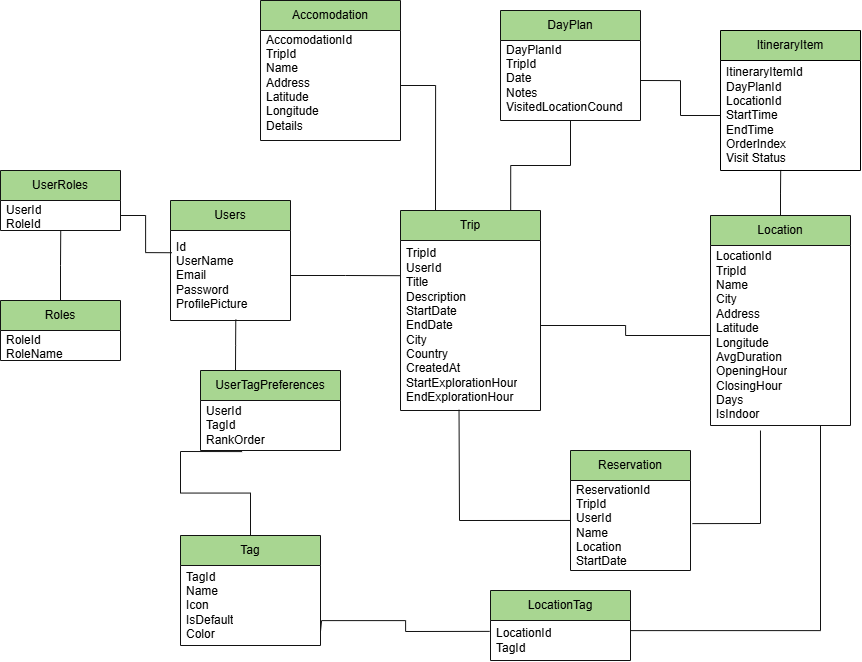
\includegraphics[width=0.7\linewidth]{Licenta.drawio.png}
    \caption{Figure}
    \label{fig:architecture_diagram}
\end{figure}

\section{Autentificare și Autorizare: ASP.NET Identity}

\subsection{Cadrul de gestionare a identității}
ASP.NET Core Identity este un sistem predefinit pentru gestionarea utilizatorilor. Adoptarea acestuia este optimă din următoarele considerente:

\begin{itemize}
    \item  hashing-ul și stocarea securizată a parolelor (folosind algoritmi de cripta adaptivi precum PBKDF2);
    \item  capacități de autentificare cu doi pași, în acest caz cu confirmarea prin e-mail;
    \item  controlul accesului bazat pe rol, activat prin intermediul AddRoles<IdentityRole>().
\end{itemize}

Integrare cu EF Core: Identity utilizează Entity Framework pentru persistența datelor, eliminând necesitatea unei biblioteci de autentificare separate și asigurând o integrare cu modelul de date al aplicației prin `IdentityDbContext<ApplicationUser>`.\href{https://arxiv.org/abs/2009.02114}{}\cite{identity_ref}

\section{Tehnologii Frontend}
\subsection{Framework-ul Bootstrap}
Bootstrap, inclus în structura proiectului sub directorul wwwroot/lib/bootstrap/, este un framework CSS esențial care furnizează un design adaptiv și asigură consistența vizuală a platformei, garantând o interfață uniformă pe toate paginile prin intermediul componentelor sale predefinite. În plus, sprijină accesibilitatea prin componentele sale implementate în conformitate cu directivele WCAG (Web Content Accessibility Guidelines). Totodată, accelerează dezvoltarea prin minimizarea codului CSS personalizat.

\subsection{jQuery și mecanismele de validare}
Biblioteca jQuery împreună cu extensiile sale dedicate validării oferă următoarele avantaje tehnice:
\begin{itemize}
    \item  validare non-intruzivă: regulile de validare sunt specificate în atributele data ale HTML, mai degrabă decât în JavaScript inline, păstrând preocupările separate;
    \item  prevenirea erorilor pe partea de client: înainte ca datele să ajungă la server, validarea pe partea clientului oferă feedback imediat utilizatorului, reducând încărcarea serverului și îmbunătățind experiența;
    \item  dacă JavaScript este dezactivat, validarea pe partea serverului funcționează în continuare, asigurând integritatea datelor.
\end{itemize}

Deși framework-urile moderne (React, Vue, Angular) ar putea înlocui jQuery, configurația actuală oferă o soluție ușoară, dovedită, care nu necesită complexitate suplimentară în fluxul de construire pentru o aplicație ASP.NET Core monolitică.

\section{Caracteristici geospațiale: Mapbox}
Mapbox este configurat ca furnizor principal de hărți\href{https://link.springer.com/chapter/10.1007/978-3-031-19594-5_2}{}\cite{mapbox_ref}. Pentru acest scenariu, Mapbox prezintă avantaje față de alte alternative deoarece:

\begin{itemize}
    \item  Eficiența costurilor: modelul de tarifare al platformei Mapbox se bazează pe utilizarea reală, ceea ce îl face rentabil pentru aplicațiile cu încărcături variabile de utilizatori. Vederile asociate permit randarea unor hărți interactive capabile să vizualizeze:
        \begin{itemize}
            \item  puncte de interes (POI) distribuite de-a lungul itinerariului;
            \item  rute și traiectorii topologice calculate între locații;
            \item  evidențierea țărilor vizitate.
        \end{itemize}
    \item  Prelucrarea datelor de geolocalizare: locațiile sunt persistente utilizând coordonate spațiale precise (latitudine și longitudine), capacitate care permite motorului Mapbox să efectueze operațiuni computaționale precum: calcularea precisă a distanțelor, optimizarea rutelor, reprezentarea vizuală a gradului de complexitate a topografiei.

\end{itemize}

\section{Servicii de e-mail: MailKit}
În contextul acestei aplicații, MailKit furnizează următoarele capabilități tehnice:

\begin{itemize}
    \item  suport extins pentru protocolul SMTP: integrarea directă cu infrastructura SMTP a platformei Gmail facilitează transmiterea automată a mesajelor pentru diferite necesități;
    \item  suportă standarde moderne de autentificare și criptare a canalelor de comunicație, garantând protecție;
    \item  serviciul EmailSender implementează interfața IEmailSender, permițând migrarea viitoare către serviciile cloud fără modificări de cod.
\end{itemize}


\chapter{Prezentare aplicație}
\section{Sign in si sign out}
Aplicația cere fiecărui utilizator să își creeze un cont pe baza unui email și a unei parole pentru folosirea funcționalităților. Fiecare cont are nevoie de confirmarea email-ului, abia după confirmare utilizatorul se poate loga și folosi aplicația.

Ecranele de sign in și sign out au atașate validări împreună cu mesaje specifice pentru fiecare caz: format incorect pentru email și parolă, parolă incorectă, user inexistent. Aplicația oferă posibilitatea deconectării și ștergerii contului, având un mesaj de avertizare că datele se vor șterge, cu verificarea parolei înainte, pentru ca ștergerea să poată fi făcută doar de utilizator.

\section{Pagina principala}
Pagina principală (home) este concepută atât ca punct de intrare pentru vizitatori, cât și ca panou de control pentru utilizatorii autentificați. Pentru utilizatorii neautentificați prezintă o pagină cu detalii despre aplicație împreună cu butoane de logare și înregistrare. După logare, pagina prezintă un mesaj de bun venit și butoane care ghidează utilizatorul să creeze o nouă călătorie sau să le vizualizeze pe cele existente.

\section{Călătoriile mele}
„My Trips" (Călătoriile mele) este pagina centrală pentru gestionarea călătoriilor unui utilizator. Călătoriile sunt separate în trei categorii distincte, în funcție de statutul lor temporal. Secțiunea „Se întâmplă acum" (Happening Now) apare doar dacă o excursie este în desfășurare și afișează călătoriile active în prezent pentru un acces mai rapid la acestea. Secțiunea „Aventuri viitoare" prezintă călătoriile care urmează în viitor în ordine calendaristică pentru a ajuta utilizatorul să vizualizeze călătoriile care urmează și pentru a se pregăti pentru ele. Ultima secțiune, „Amintiri de călătorie" (Travel Memories), păstrează câteva călătorii terminate, permițând utilizatorului să vizualizeze excursiile trecute împreună cu detaliile acestora, având la dispoziție un buton de „see more" pentru a accesa o pagină cu toate călătoriile terminate.

Fiecare călătorie apare ca un card interactiv care afișează informațiile cheie, cum ar fi data și destinația. În cazul primelor două secțiuni, cardurile au atașate butoane către adăugarea de atracții, cât și un buton pentru generarea de itinerariu și vederea tuturor detaliilor. În ultima secțiune butonul de adăugare este eliminat și rămâne doar cel pentru vizualizarea detaliilor.

Un buton „Create new trip" (Creează o nouă călătorie) permite utilizatorilor să acceseze ușor crearea unei noi călătorii.

\section{Creare călătorie}
Pagina „Plan new trip" (Creează o nouă călătorie) conține un formular complet prin care utilizatorii pot crea o nouă călătorie. În formular utilizatorii introduc informații precum numele, o descriere în cazul în care aceștia doresc, destinația, datele de început și sfârșit. De asemenea formularul include selectoare pentru orele pe care utilizatorul ar vrea să le folosească pentru vizitare, folosite la generarea itinerariului. Validarea formularului asigură integritatea datelor înainte de terminare, ajutând utilizatorul să completeze corect câmpurile. Această pagină este primul pas în procesul de planificare a călătoriei și este baza pentru următorii pași.

\section{Detaliile călătoriei}
Pagina „Details" (Detalii) este cea mai cuprinzătoare și include cele mai multe funcții din aplicație, concepută pentru a oferi o imagine de ansamblu completă și o interfață de gestionare a unei călătorii. Pagina prezintă informația defalcată în două secțiuni pentru o înțelegere mai clară a acesteia.

Coloana din stânga prezintă toate detaliile călătoriei selectate. În partea de sus avem o listă colapsabilă cu toate locațiile adăugate și cele două butoane de generare. Opțional, utilizatorul poate adăuga adresa cazării în care va sta, care va apărea pe hartă pentru o mai bună generare a itinerariului. Odată ce itinerariul este generat, în secțiunea „Daily itinerary" se afișează o listă cu fiecare zi din excursia selectată și un orar cu locațiile asociate acelei zile. Fiecare locație are o casetă de selectare unde utilizatorul poate bifa locațiile vizitate.

Coloana din dreapta prezintă o hartă interactivă generată prin Mapbox în care putem vizualiza traseul geografic al călătoriei. În această hartă sunt afișate toate locațiile prin pinuri pe hartă. După generarea traseului, aceste locații sunt conectate prin rute de culori diferite în funcție de ziua din care fac parte, pentru o mai bună vizualizare spațială și temporală a fiecărei zile.

\subsection{Generare simpla a itinerariului}
Funcția „GenerateItinerary" (Generare itinerariu) este construită pe o euristică Greedy Nearest-Neighbor modificată, o abordare derivată din Problema Comis Voiajorului (TSP). În forma canonică, algoritmul Nearest-Neighbor începe de la un nod dat și selectează în mod repetat cel mai apropiat nod nevizitat până când toate nodurile au fost vizitate. În implementarea noastră, acest concept a fost adaptat pentru a funcționa în cadrul constrângerilor creării unui itinerariu de călătorie pe mai multe zile, unde ferestrele de timp, rezervările, disponibilitatea locației și preferințele utilizatorului trebuie respectate simultan.

\ding{117}{Ce am modificat}

Algoritmul standard Nearest-Neighbor funcționează exclusiv pe distanță, alege cel mai apropiat punct nevizitat geografic la fiecare pas. Versiunea noastră înlocuiește distanța geografică brută cu timpul real de călătorie, obținut din API-ul Mapbox Directions Matrix, care returnează duratele reale de mers pe jos și cu mașina între poziția curentă și toate destinațiile candidate. La fiecare pas algoritmul încearcă să găsească cea mai apropiată locație din punct de vedere temporal, încadrându-se în fereastra de timp disponibilă. Această schimbare este importantă deoarece două locații echidistante pe hartă pot avea timpi diferiți de călătorie în funcție de drumurile parcurse.

Deoarece în aplicația noastră apar restricții de timp, vom introduce un concept de constrângeri temporale având atât rezervări (rezervări externe fixe cu ore de început și sfârșit), cât și elemente vizitate (locații pe care utilizatorul le-a vizitat). În faza de curățare, elementele vizitate sunt relocate, astfel încât următoarele zile să fie reconstruite de la zero. Într-o anumită zi, la fiecare iterație, algoritmul analizează în perspectivă următorul eveniment fix. Înainte de a plasa o locație nouă în program, algoritmul verifică dacă utilizatorul ar avea suficient timp pentru a ajunge acolo, a petrece durata medie și a ajunge la următorul eveniment cu o marjă de eroare de 15 minute. Se încearcă până se găsește o locație care poate respecta aceste condiții, pentru a evita crearea unui conflict cu o rezervare preexistentă.

\ding{117}{Ce folosește algoritmul pentru a calcula}

Fiecare iterație procesează fiecare DayPlan cronologic. Pentru fiecare zi, bucla inițiază un cursor currentTime la ora configurată de începere a explorării și un cursor endTimeLimit la ora de sfârșit a explorării. Dacă cazarea a fost adăugată, aceasta este ancorată ca poziție de începere, astfel încât prima iterație în fiecare zi începe de la cazare. Bucla apelează apoi FindBestNextLocationAsync.

În interiorul acestei funcții, se verifică dacă există mai mult de 24 de locații candidate. Dacă da, acestea sunt prefiltrate folosind formula Haversine, care calculează distanța dintre două coordonate geografice ținând cont de curbura planetei, pentru a selecta doar cele 24 de locații cele mai apropiate. Aceasta este o optimizare necesară deoarece API-ul Mapbox Matrix are o limită de 25 de puncte per solicitare, astfel încât prefiltrul Haversine acționează ca o modalitate ușoară și rapidă de a elimina locațiile prea îndepărtate înainte de a efectua apelul API. Calculul Haversine convertește diferențele de latitudine și longitudine în radiani, aplică legea sferică a cosinusurilor prin termenii sin² și cos și returnează distanța în metri prin raza Pământului de 6.371.000 de metri.

Odată ce lista de candidați a fost redusă, funcția apelează API-ul Mapbox Matrix de două ori în paralel, o dată pentru durata de mers pe jos și o dată pentru durata de condus între poziția curentă și toți candidații. Pentru fiecare candidat algoritmul alege care este cel mai rapid mijloc de a ajunge în acea locație. Dacă API-ul eșuează sau nu returnează niciun rezultat pentru un anumit candidat, algoritmul revine la un timp de călătorie estimat calculat din distanța Haversine împărțind la o viteză medie de 10 km/h, aproximând un ritm de mers rapid. Această soluție asigură că algoritmul nu se oprește din cauza defecțiunilor rețelei.

Pentru fiecare candidat, algoritmul aplică două filtre înainte de a-l considera cea mai bună alegere. Primul filtru este IsLocationOpen, care verifică orele de deschidere și închidere ale locației în raport cu ora de sosire proiectată. Al doilea este FitsBeforeNextEvent, care verifică dacă vizita completă a locației, sosirea plus durata medie, se încheie în timp util pentru a ajunge la următoarea locație; în cazul rezervărilor această constrângere este mărită cu 15 minute. Candidații care trec de ambele filtre sunt luați în considerare, fiind ales cel care are cel mai scurt timp de călătorie, păstrând regulile algoritmului Greedy.

Algoritmul rezolvă și problema schimbărilor în itinerariu, atunci când utilizatorul nu reușește să viziteze totul dintr-o anumită zi sau înregistrează o locație înainte de program. În loc să permită blocarea programului unei întregi zile, detectează locațiile care au fost vizitate înainte și le mută în ziua curentă din baza de date. Istoricul locației este păstrat, dar ziua viitoare este eliberată astfel încât itinerariul să poată fi regenerat. După curățare, algoritmul construiește setul de locații încă disponibile pentru programare prin interogarea elementelor itinerariului și colectarea celor marcate „Vizitate". Acestea, împreună cu orice rezervare, sunt ulterior excluse din grupul de candidați, rămânând doar locațiile care pot fi reprogramate.

Această strategie de regenerare face ca algoritmul să fie idempotent și sigur pentru a putea fi rulat din nou. Nu există riscul ștergerii istoricului sau completării retroactive a unei zile deja trecute.

\subsection{Generare cu ai}
Funcția GenerateWithAI implementează un model fundamental diferit: nu este un algoritm de rutare în sine, ci mai degrabă o conductă în două etape care combină un LLM pentru descoperirea semantică a locurilor cu API-ul de Geocodare Mapbox pentru validarea coordonatelor din lumea reală, urmată de un apel recursiv către GenerateItinerary pentru a programa efectiv locațiile nou găsite.

\ding{117}{Solicitarea LLM bazate pe preferințe}

Prima etapă interoghează preferințele de etichete stocate ale utilizatorului din baza de date, preluând categoriile pe care le-a clasificat. Acestea sunt transmise într-o solicitare structurată trimisă modelului LLaMA 3.3 70B prin intermediul API-ului Groq. Modelul este solicitat cu o instrucțiune de sistem constrânsă: trebuie să răspundă doar într-o schemă JSON specifică care conține o matrice de obiecte, fiecare cu un nume și o etichetă. Partea de solicitare orientată către utilizator solicită până la 8 locuri de interes reale, vizitabile, în orașul și țara călătoriei sau în apropiere, prioritizate în funcție de etichetele principale ale utilizatorului și exclude în mod explicit hoteluri, restaurante și cartiere.

Răspunsul modelului este analizat, iar șirul JSON brut este curățat prin găsirea primelor caractere `{}` și extragerea datelor, măsură care asigură evitarea oricărui preambul sau text final pe care modelul l-ar putea produce în ciuda solicitării stricte.

\ding{117}{Validarea}

Deoarece LLM-ul poate halucina unele nume sau poate returna locații din orașul greșit, fiecare sugestie returnată de model este validată independent prin intermediul API-ului Mapbox Search Forward Geocoding. Pentru fiecare nume de loc sugerat, funcția construiește o interogare de geocodare care combină numele locului cu orașul călătoriei și adaugă o verificare de proximitate folosind coordonatele centrului geografic al orașului. Această verificare este necesară pentru a returna doar rezultate din interiorul orașului sau din apropierea orașului, mai degrabă decât un loc cu același nume din altă parte.

Fiecare rezultat de geocodare este supus unor filtre de validare. Numele este verificat în raport cu o listă de cuvinte cheie precum „hotel", „apartament", „parcare" și altele asemenea, pentru a nu intra în itinerariu. Adresa rezultatului este verificată pentru a confirma că menționează țara și orașul corect. Dacă numele orașului nu apare în adresă, se aplică o verificare de proximitate prin formula Haversine pentru a calcula distanța dintre coordonatele rezultatului și centrul orașului, iar rezultatele aflate pe o rază de 30 de km sunt acceptate chiar dacă numele lipsește din textul adresei. Aceasta gestionează cazurile în care o excursie este planificată într-o locație mică, unde locațiile ar putea fi situate adiacent. În cele din urmă, rezultatul este verificat atât în raport cu locațiile deja existente, cât și cu cele deja adăugate, pentru a preveni intrările duplicate. Pentru fiecare locație se creează o nouă entitate Locație care se adaugă în baza de date.

Odată ce toate locațiile au fost salvate, GenerateWithAI se termină cu un apel către GenerateItinerary, deoarece funcția AI este un mecanism de descoperire și populare cu locații, în timp ce algoritmul propriu-zis de generare se află exclusiv în GenerateItinerary. Cele două generări au în comun un singur motor de programare unificat, astfel încât îmbunătățirile uneia o avantajează și pe cealaltă.

\section{Adăugare obiective}
„Add Location" (Adăugare locații) permite utilizatorilor să adauge puncte de interes în itinerariul călătoriei alese. În stânga se află harta interactivă unde fiecare locație adăugată este evidențiată printr-un pin colorat specific etichetelor din care face parte. De asemenea se pot selecta manual locații direct din hartă și ulterior se pot adăuga în listă, sau se pot căuta orice locații folosind bara de căutare de deasupra hărții. Aceasta folosește cuvinte cheie introduse și oferă variante care se potrivesc. Odată ce o locație este selectată, pinul va apărea pe hartă, iar în dreapta secțiunea „Add new" se va completa cu datele acelei locații. Pentru fiecare locație sunt prezentate numele și locația, o listă de etichete care îi sunt asociate. De asemenea avem câmpuri suplimentare cu durata aproximativă de vizitare și orele în care această locație este deschisă, acestea autocompletându-se dar cu posibilitatea de editare. Apăsând pe butonul „Add to itinerary" (Adaugă în itinerariu), pinul se colorează corespunzător și locația rămâne salvată în listă.

Secțiunea de sugestii este o funcție de recomandări concepută pentru a ajuta utilizatorii să descopere atracții și puncte de interes din orașul pe care îl vizitează. Meniul este organizat pe categorii, cu un meniu derulant care oferă diverse opțiuni, cum ar fi Muzee, Parcuri, Restaurante, Atracții și multe altele. Utilizatorii pot alege variante aleatoare pentru a obține o colecție diversă de locuri sau pot alege o categorie specifică. Când o locație este accesată, toate specificațiile vor apărea în pagina de adăugare.

Ultima secțiune este lista de locații pe care utilizatorul le are adăugate în călătoria curentă. Aceasta este o vizualizare rapidă a tuturor locațiilor, fiecare apărând într-un card interactiv care afișează toate detaliile. Dacă utilizatorul apasă pe un card, harta se va centraliza pe acea locație și detaliile vor apărea în pagina de adăugare. Fiecare card are un buton de ștergere și unul de „Add Event" (Adaugă eveniment), care dacă este apăsat va deschide un card unde se pot adăuga detaliile unui eveniment care va avea loc la acea locație: numele, ora începerii și durata.

\section{Pagina calendar}
Pagina „Calendar" (Calendar) prezintă un cuprins al tuturor călătoriilor unui utilizator într-un format de calendar, oferind o imagine de ansamblu rapidă asupra programului de călătorie pe tot parcursul anului. Fiecare călătorie este evidențiată, facilitând identificarea momentului când are loc o călătorie și planificarea în funcție de acestea. Utilizatorii pot naviga între vizualizare pe luni sau ani, iar apăsând pe o anumită călătorie sunt redirecționați rapid la pagina cu detalii corespunzătoare. Această vizualizare ajută utilizatorii să își organizeze mai bine excursiile pe parcursul anului și oferă o imagine de ansamblu a acestora.

\section{Harta interactivă}
„ScratchMap" (Harta Răzuibilă) este o funcție de gamificare care afișează o hartă interactivă a lumii ce evidențiază toate țările vizitate anterior și cele care vor urma. Pe măsură ce utilizatorii creează și finalizează călătorii, țările sunt evidențiate automat în culori distincte pe hartă, verde pentru cele terminate și galben pentru cele care vor urma, creând o imagine de ansamblu vizuală a explorării globului. Această funcție oferă o vizualizare captivantă a istoricului călătoriilor, aliniindu-se cu obiectivul aplicației de a face planificarea călătoriilor mai plăcută.

\section{Pagina de preferințe}
În pagina „My preferences" (Preferințele mele) utilizatorul își poate configura interesele și prioritățile, care servesc ca bază pentru algoritmul de recomandare bazat pe inteligența artificială. Pagina prezintă o colecție cuprinzătoare de categorii și etichete de interes organizate pe trei niveluri de prioritate. Interacțiunea cu acestea se face printr-o interfață intuitivă care permite glisarea și plasarea etichetelor în unul din cele trei niveluri de prioritate. Acest sistem este util în generarea itinerariilor, algoritmul ponderând recomandările în funcție de aceste priorități, asigurându-se că planurile de călătorie se aliniază cu interesele fiecărui utilizator.

\chapter{Concluzii și perspective de dezvoltare}

\section{Concluzii}
Prin prezenta lucrare am abordat dezvoltarea unei aplicații de planificare a călătoriilor, concepută pentru a facilita procesul organizării unui itinerariu complex. Aplicația integrează cu succes mai multe tehnologii și caracteristici într-o platformă care ușurează experiența de planificare.

\begin{itemize}
    \item Dezvoltarea unui algoritm care colectează preferințele utilizatorilor și generează itinerarii personalizate pe baza acestora. Această abordare depășește simplele sugestii de „cele mai vizitate atracții” și oferă o experiență personalizată fiecărui utilizator.
    \item Centralizarea tuturor informațiilor (rezervări, cazări, locații) într-o singură platformă. Acest lucru elimină dificultatea jonglării cu mai multe aplicații și a gestionării logisticii.
    \item Capacitatea sistemului de a actualiza itinerariile, permițând utilizatorilor să bifeze locațiile vizitate și să regenereze planurile rămase pe baza progresului real. Replanificarea asigură o planificare optimă a traseului pe tot parcursul călătoriei.
\end{itemize}

\section{Perspective de dezvoltare}
În ceea ce privește perspectivele de dezvoltare, aplicația are numeroase posibilități de extindere:

\begin{itemize}
    \item Integrarea modelelor de învățare automată pentru a prezice timpii optimi de călătorie pe baza datelor istorice sau pe baza traficului în timp real, oferind astfel o planificare și mai precisă.
    \item Analiza predictivă pentru a sugera destinații pe baza modelelor de comportament ale utilizatorilor și a experiențelor similare de călătorie.
    \item Planificarea colaborativă pentru scenarii de călătorie în grup, cu recomandări comune.
    \item Integrarea cu servicii meteo pentru prognoza meteo în timp real și recomandări de călătorie.
    \item Servicii bazate pe locație și geofencing pentru a oferi memento-uri, informații și autocompletarea itinerariului în timp real.
    \item Integrarea calculării rutelor folosind transportul public sau alte opțiuni de transport pentru a oferi o planificare completă a călătoriei.
\end{itemize}

\nocite{dotnet_aspnet}
\printbibliography[heading=bibintoc]

\end{document}

